\paragraph{} O método aplicado a este trabalho pode ser dividido em 5 etapas principais, se dividindo entre desenvolvimento e teste. Inicia-se pela coleta de dados, a partir de fontes abertas e confiáveis, seguido pela etapa de divisão do conjunto de dados em desenvolvimento e teste, etapas de pré-processamento, onde características principais são extraídas antes do treinamento de um modelo neural e por fim, a avaliação dos modelos no conjunto de desenvolvimento, para a escolha de hiperparâmetros e no conjunto de teste, para avaliar a capacidade de generalização. O diagrama de processamento do método é mostrado na Figura \ref{fig:processamento_diagram} e o método detalhado nas seções a seguir.

\begin{figure}
	\begin{center}
		\begin{center}
			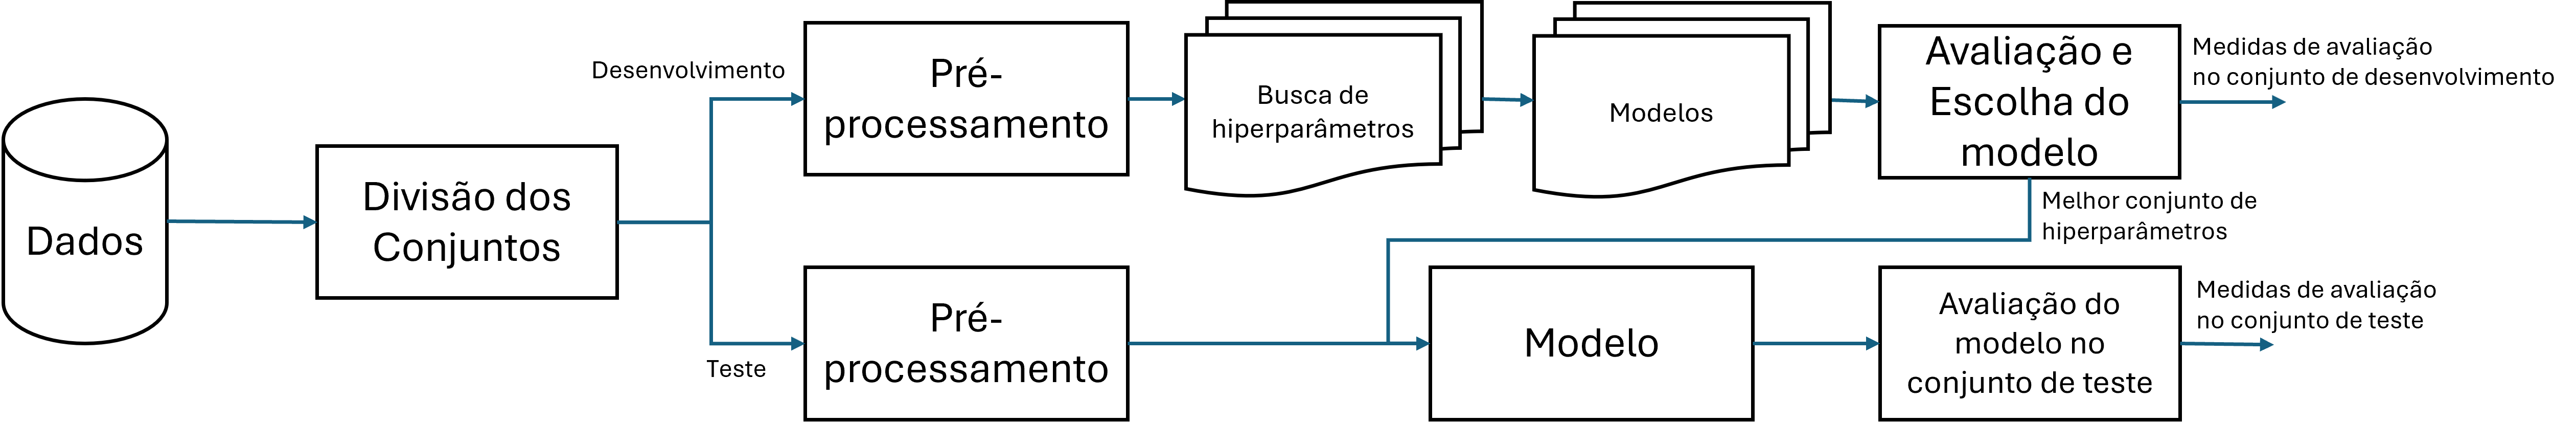
\includegraphics[width=\textwidth]{figuras/processamento_diagram.png}
			\caption{Fluxo de Processamento}
			\label{fig:processamento_diagram}
		\end{center}

	\end{center}
\end{figure}

\section{Coleta de Dados}

\paragraph{} A primeira etapa deste trabalho é a coleta de dados, que é uma etapa importante para a construção de um modelo de previsão. A qualidade dos dados coletados influencia diretamente a qualidade do modelo. Para este trabalho, os dados foram coletados de fontes públicas e confiáveis, como a \ac{ANP} (em conformidade com a Lei de Acesso a Informação \cite{lei12527}), o Banco Mundial e o Index Mundi. O intervalo de tempo escolhido para a análise compreende o período entre janeiro de 2022 e julho de 2023, permitindo a avaliação da série em 2 períodos sazonais para uma previsão no curto prazo.
\paragraph{} Além disso, serão usados como covariáveis passadas as séries de preços do Óleo de Soja Internacional e do Óleo de Soja no Mercado Futuro. Para possibitar uma análise de um período de tempo maior, as séries de preços do Óleo de Soja Internacional e do Óleo de Soja no Mercado Futuro foram coletadas desde 1960 e 1994, respectivamente.
\paragraph{} A seleção das séries temporais foi baseada na disponibilidade de dados históricos e na correlação observada entre elas durante o período de análise, conforme ilustrado na Figura \ref{fig:correlation_matrix}. A alta correlação entre as séries regionais de preços do biodiesel sugere que a inclusão dessas séries no modelo não contribui com informações adicionais relevantes.
\paragraph{} De maneira semelhante, as covariáveis foram escolhidas com base em critérios de correlação. A série de preços do óleo de soja internacional demonstra uma alta correlação com as séries de preços do biodiesel, tornando-a uma candidata promissora para o treinamento do modelo devido à maior disponibilidade de dados. Por outro lado, a série de preços do óleo de soja no mercado futuro também apresenta alta correlação com as séries de preços do biodiesel. No entanto, como essa série tem uma correlação perfeita com a série de preços do óleo de soja internacional, sua inclusão no modelo não adiciona valor informativo adicional.
\paragraph{} Portanto, as séries escolhidas para treinamento do modelo são: Preço do Biodiesel Nacional e Preço do Óleo de Soja Internacional.

\begin{figure}
	\begin{center}
		\begin{center}
			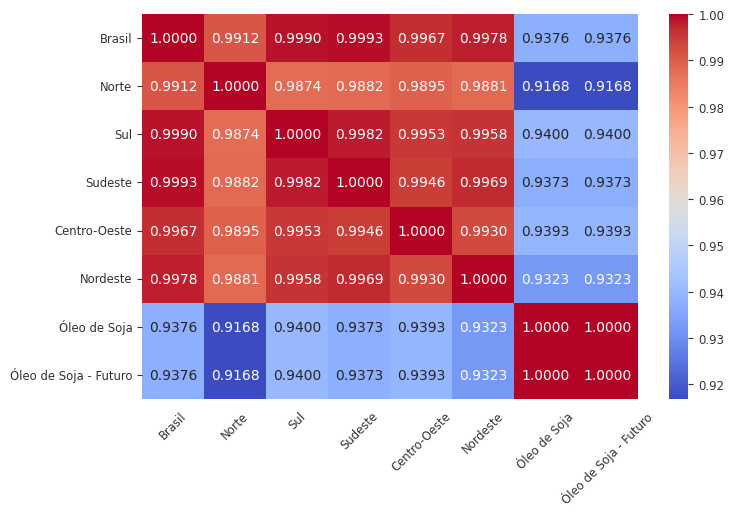
\includegraphics[width=0.8\textwidth]{figuras/correlation_matrix.png}
			\caption{Matriz de Correlação entre as Séries Candidatas (01/2022 - 07/2023)}
			\label{fig:correlation_matrix}
		\end{center}

	\end{center}
\end{figure}

\section{Divisão do Conjunto de Dados}
\paragraph{} Para uma modelagem e avaliação mais eficaz do modelo, os dados foram divididos em dois conjuntos: desenvolvimento e teste, conforme mostrado na Figura \ref{fig:series_conjunto_timeline}.
\paragraph{} O período até julho de 2023 foi alocado para o conjunto de desenvolvimento, que é utilizado para ajustar os hiperparâmetros do modelo e validar sua eficácia. Esse conjunto inclui dados suficientes para observar a dinâmica sazonal e garantir a capacidade de generalização do modelo. Os dados restantes são usados como conjunto de teste, fornecendo uma avaliação final não tendenciosa do modelo com dados que não foram vistos anteriormente. Este modelo de divisão é uma prática recomendada pela literatura para garantir confiabilidade e robustez do modelo de previsão \cite{saha2024}.

\begin{figure}
	\begin{center}
		\begin{center}
			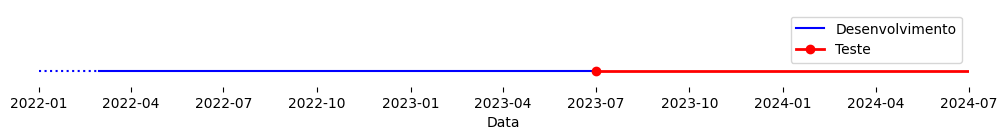
\includegraphics[width=\textwidth]{figuras/series_conjunto_timeline.png}
			\caption{Linha do Tempo da Divisão dos Conjuntos}
			\label{fig:series_conjunto_timeline}
		\end{center}

	\end{center}
\end{figure}


\section{Pré-processamento dos Dados}
\paragraph{} Após a divisão dos conjuntos, é aplicado o processo de pré-processamento. Que pode ser subdividido em em 4 partes principais: Processo de descorrelação, divisão em janelas temporais, extração de características e escalamento do resíduo, como mostrado na Figura \ref{fig:preprocessamento_diagram}.

\begin{figure}
	\begin{center}
		\begin{center}
			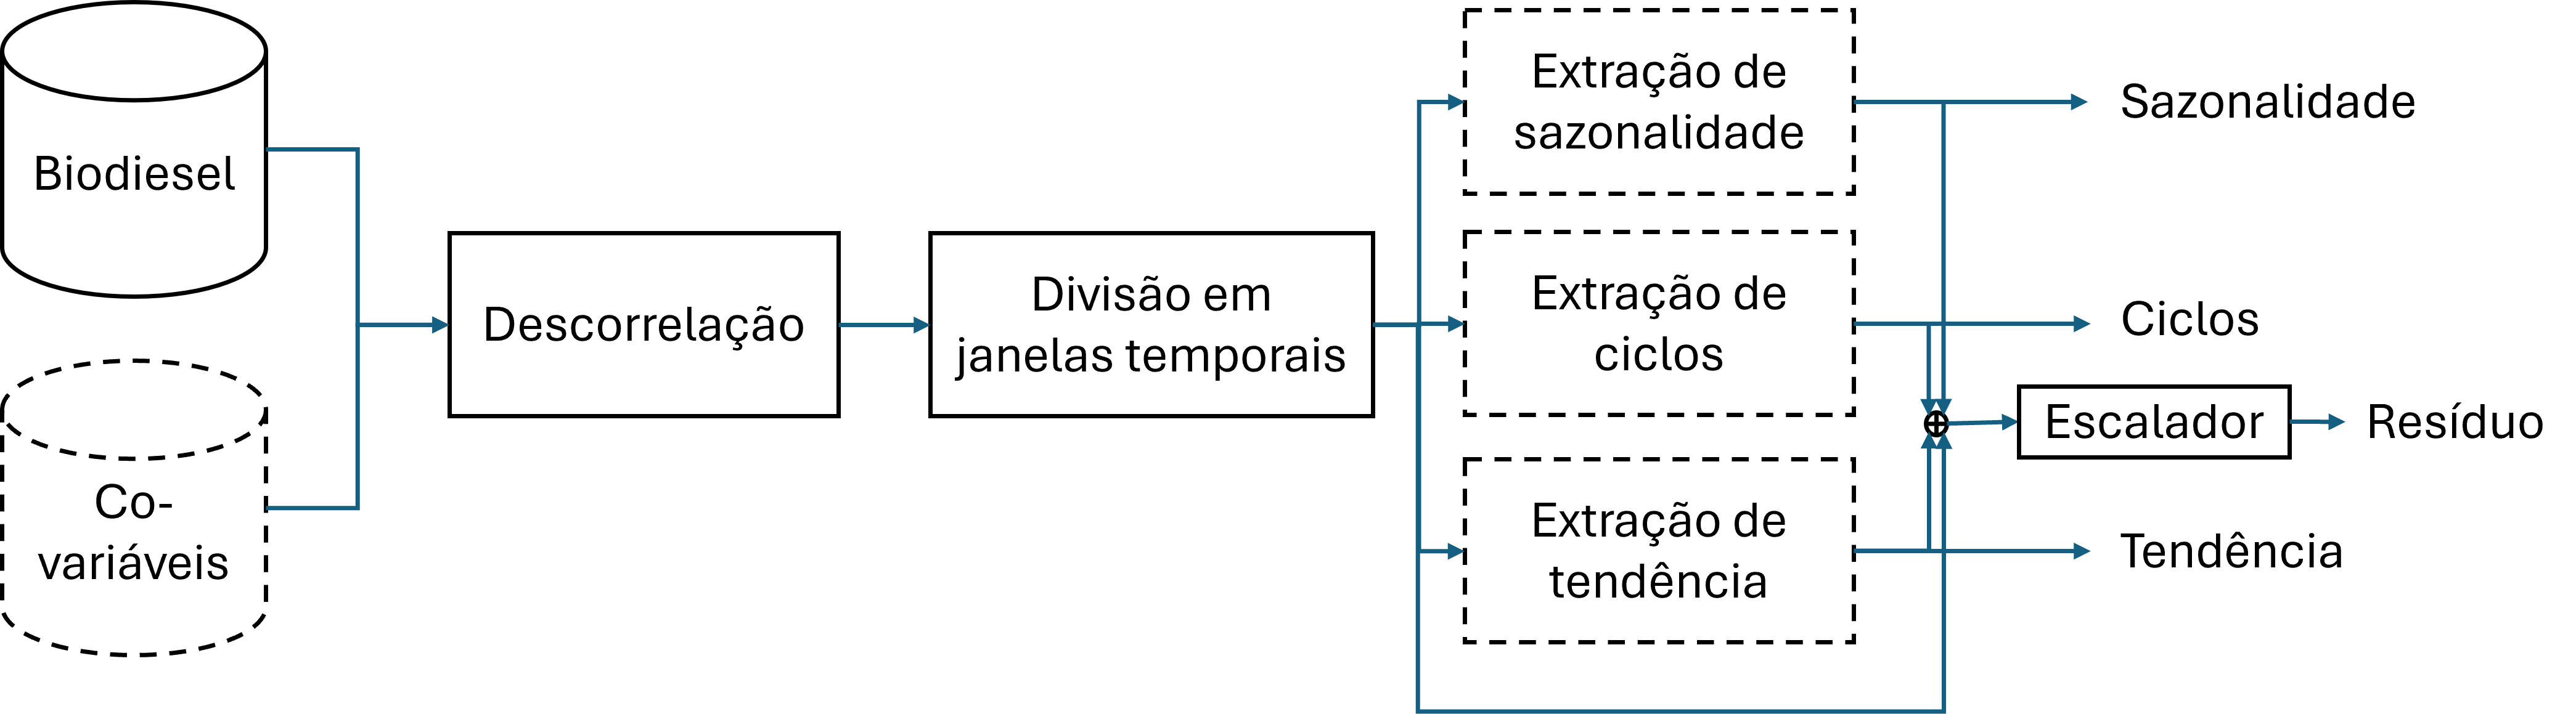
\includegraphics[width=\textwidth]{figuras/preprocessamento_diagram.png}
			\text{---: Obrigatório} \\
			\text{- -:  \space \space \space Opcional}
			\caption{Fluxo de Pré-Processamento}
			\label{fig:preprocessamento_diagram}
		\end{center}

	\end{center}
\end{figure}

\paragraph{} Inicialmente, o conjunto de desenvolvimento foi submetido a uma análise para identificar padrões de sazonalidade e ciclos senoidais. Caso sejam identificados, o tamanho da janela temporal deve ser escolhido de modo a capturar pelo menos 2 observações de cada padrão.
\paragraph{} A verificação da sazonalidade foi realizada por meio da autocorrelação da série temporal. No entanto, a análise não revelou ciclos sazonais completos, conforme ilustrado na Figura \ref{fig:acf_biodiesel}. Além disso, para identificar ciclos senoidais, foi empregada a Transformada Rápida de Fourier (FFT). No entanto, a análise de FFT também não conseguiu identificar ciclos senoidais significativos na série temporal, como mostrado na Figura \ref{fig:fft_biodiesel}. Esses resultados indicam a ausência de padrões sazonais e cíclicos evidentes nos dados analisados.

\paragraph{} A verificação da persistência foi realizada utilizando o Coeficiente de Hurst, conforme descrito na Equação \ref{eq:hurst}. Essa abordagem permite analisar a série temporal para verificar se ela exibe um comportamento de persistência, o que significa que os valores futuros podem ser previstos a partir dos dados passados.
\paragraph{} Com base nessa análise, obteve-se um Coeficiente de Hurst igual a 0,73, constatou-se que a série apresenta um comportamento de persistência, o que implica uma correlação positiva entre os valores atuais e os valores passados. Em outras palavras, quando a série tende a aumentar, as tendências passadas indicam uma probabilidade de continuar subindo, e quando tende a cair, as tendências passadas sugerem uma continuidade desse movimento. Isso reforça a possibilidade de previsão a partir de dados históricos, validando a hipótese de dependência de longo prazo na série temporal.

\begin{figure}
	\begin{center}
		\begin{center}
			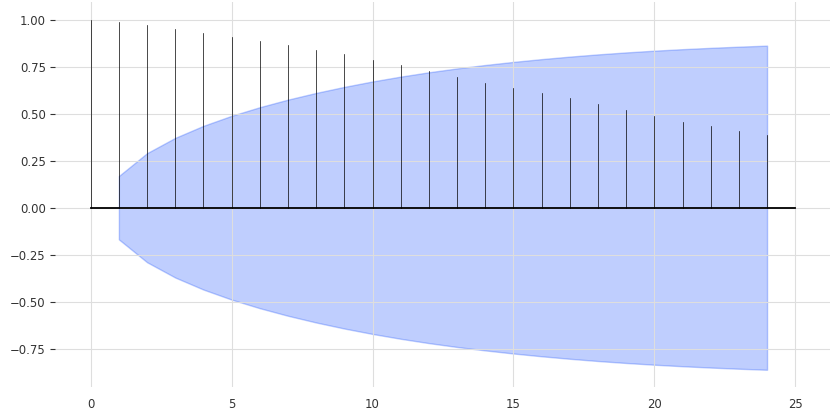
\includegraphics[width=0.8\textwidth]{figuras/acf_biodiesel.png}
			\caption{Autocorrelação da Série de Preços do Biodiesel}
			\label{fig:acf_biodiesel}
		\end{center}

	\end{center}
\end{figure}

\begin{figure}
	\begin{center}
		\begin{center}
			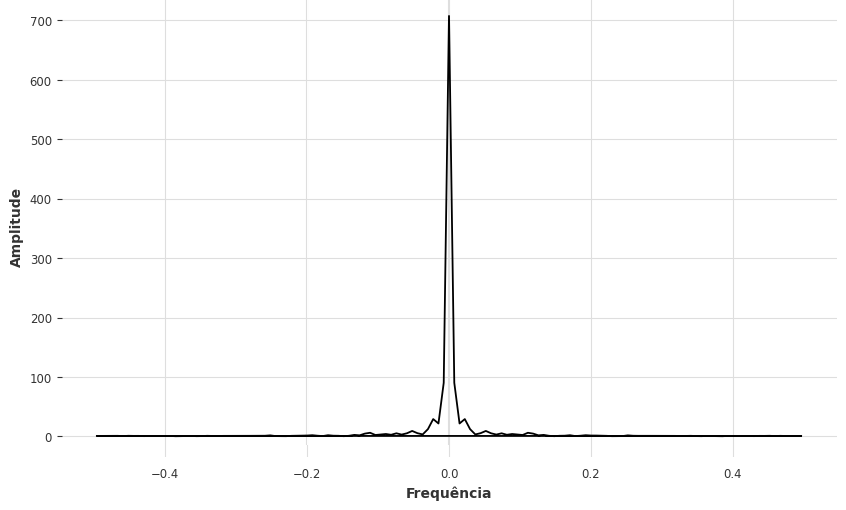
\includegraphics[width=0.8\textwidth]{figuras/fft_biodiesel.png}
			\caption{Frequências de Fourier da Série de Preços do Biodiesel}
			\label{fig:fft_biodiesel}
		\end{center}

	\end{center}
\end{figure}
\paragraph{} Os dados selecionados, o preço do biodiesel nacional e do óleo de soja internacional, foram submetidos a um processo de descorrelação para remover dependências lineares entre as variáveis, como mostrado na matriz de correlação da Figura \ref{fig:correlation_matrix}, removendo os dados da série do óleo de soja internacional no período em que há dados das duas séries, como mostrado na Figura \ref{fig:series_timeline}. Em seguida, os dados foram divididos em dois experimentos distintos. O primeiro experimento considera apenas o preço do biodiesel nacional, enquanto o segundo experimento incorpora tanto o preço do biodiesel quanto o preço do óleo de soja, permitindo a análise do impacto combinado dessas variáveis nos modelos de previsão.

\begin{figure}
	\begin{center}
		\begin{center}
			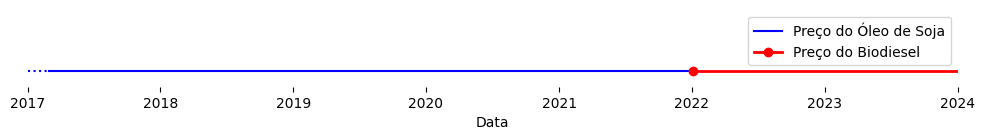
\includegraphics[width=\textwidth]{figuras/series_timeline.png}
			\caption{Linha do Tempo dos Períodos de Disponibilidade das Séries de Biodiesel e Óleo de Soja}
			\label{fig:series_timeline}
		\end{center}

	\end{center}
\end{figure}

\paragraph{} Posteriormente, os dados foram segmentados em janelas temporais, aplicando duas abordagens previamente descritas na fundamentação teórica: (1) Janela Deslizante com sobreposição, que permite capturar a continuidade temporal ao criar séries sobrepostas; e (2) Janela de Takens, que reconstrói o espaço de estados da série temporal a partir de um único sinal, utilizando atrasos específicos para capturar as dinâmicas subjacentes.
\paragraph{} Foram aplicadas duas abordagens distintas para a normalização e decomposição dos dados. Na primeira abordagem, os dados brutos foram normalizados diretamente utilizando a Equação \ref{eq:normalization-min-max}. Na segunda abordagem, os dados foram primeiramente processados para remover a tendência linear, ajustada pela Equação \ref{eq:linear-regression}, resultando em dados residuais. Esses dados residuais foram então normalizados utilizando novamente a Equação \ref{eq:normalization-min-max}.

\section{Treinamento e Avaliação dos Modelos}
\paragraph{} Em seguida, foi realizada a validação cruzada para avaliar o desempenho do modelo de forma mais robusta, assegurando sua eficácia e confiabilidade em diferentes subconjuntos de dados.
\paragraph{} O conjunto de desenvolvimento é dividido em 2 subconjuntos. O conjunto de treinamento, usado para apresentar amostras de pares entrada e saída para o modelo e o conjunto de validação usado para avaliar o modelo em dados que não foram usados para o ajuste de parâmetros, evitando sobreajuste e garantindo a capacidade de generalização. Os conjuntos são divididos com tamanhos diferentes em cada dobra da validação cruzada, conforme mostrado na Figura \ref{fig:validacao_cruzada_teo}.

\begin{figure}
	\begin{center}
		\begin{center}
			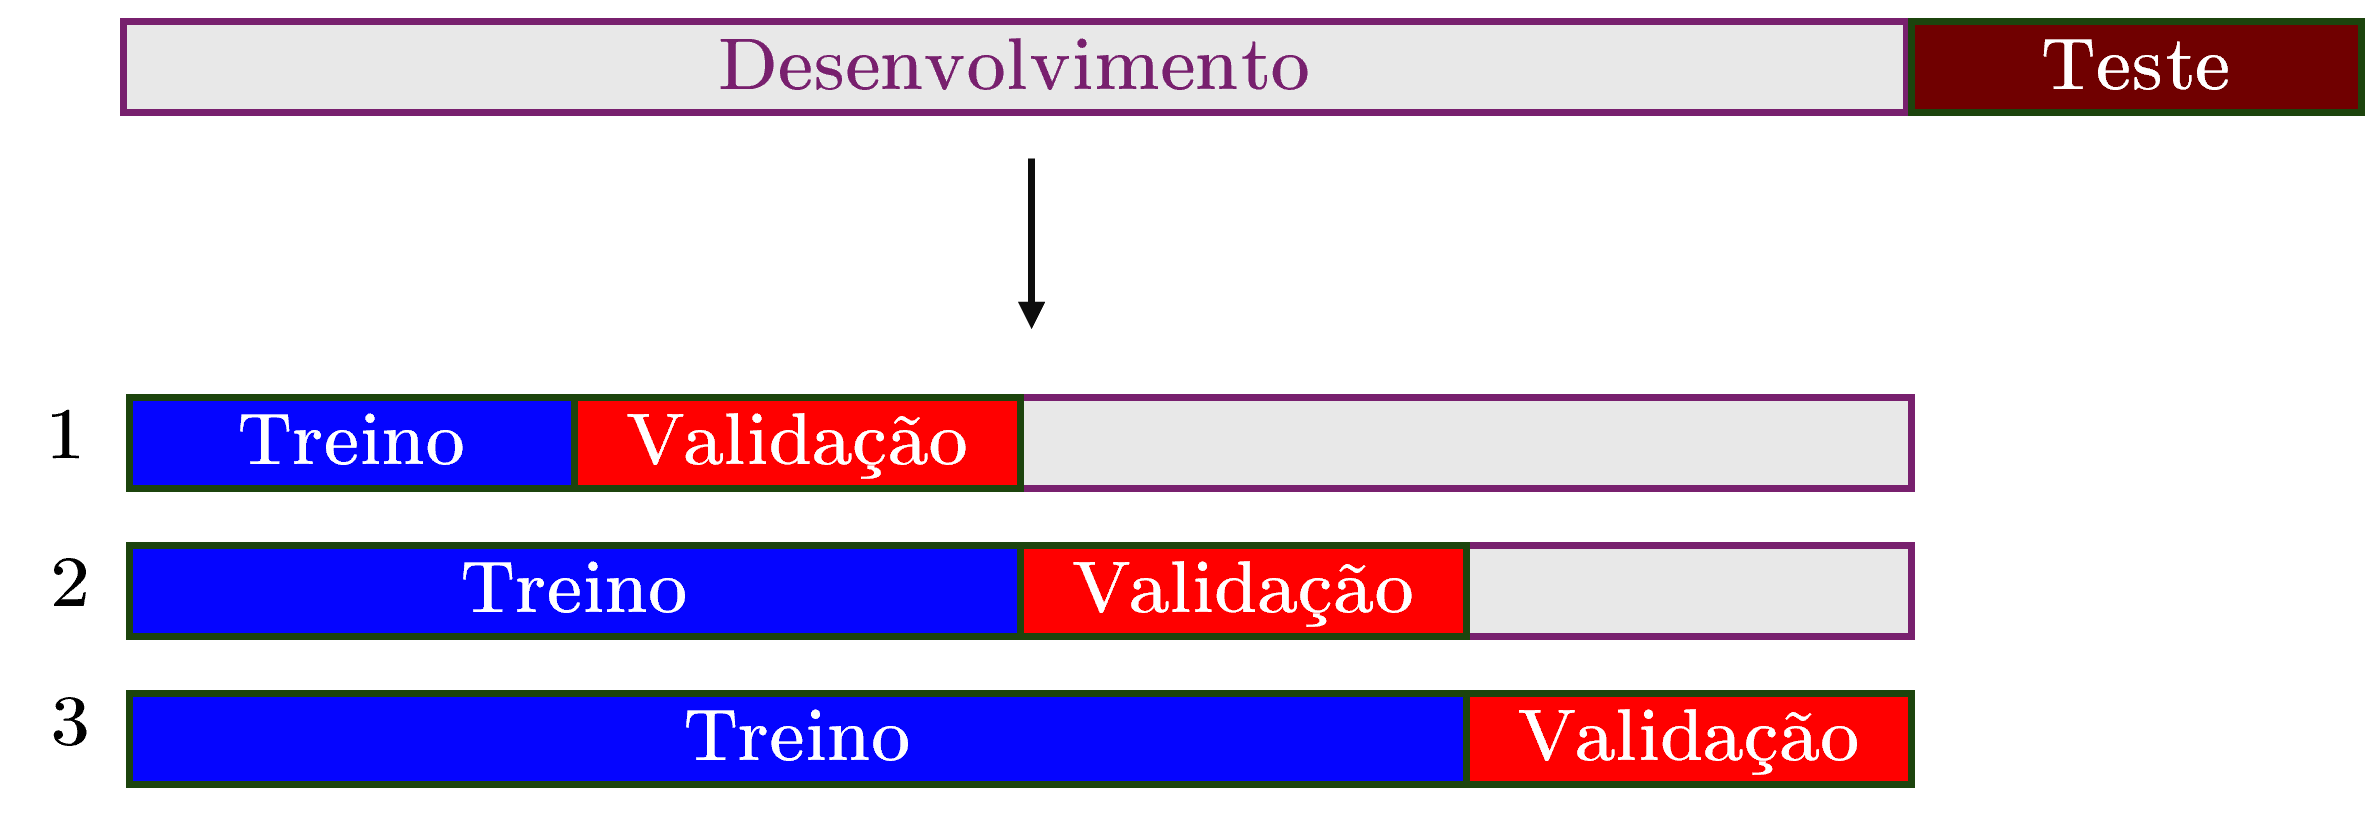
\includegraphics[width=\textwidth]{figuras/validacao_cruzada_teo.png}
			\caption{Validação Cruzada com 3 dobras}
			\label{fig:validacao_cruzada_teo}
		\end{center}
		\text{Fonte: Elaborado pelo autor, baseado em \cite{hyndman2018forecasting}}

	\end{center}
\end{figure}

\paragraph{} Após a subdivisão, os modelos serão treinados usando o conjunto de treinamento e seu desempenho será avaliado pelas medidas de desempenho: \ac{MAPE}, \ac{SLE}, \ac{MSE}, \ac{RMSE}, \(U_1\) e \(U_2\) de cada conjunto de validação e com os resultados serão calculados média e desvio padrão para cada medida. O melhor conjunto de hiperparâmetros será escolhido pelo algoritmo Optuna \cite{optuna_2019} e o ajuste fino será feito pela GridSearch.

\paragraph{} Após a definição dos hiperparâmetros com base nas medidas de desempenho, o modelo será treinado usando todo o conjunto de desenvolvimento e, em seguida, avaliado no conjunto de teste. Isso permitirá verificar sua capacidade de generalização para dados que não foram vistos anteriormente.